\documentclass[journal]{IEEEtran}

\usepackage{graphicx}
\usepackage{amsmath}
\usepackage{amssymb}
\usepackage{booktabs}
\usepackage{multirow}
\usepackage{hyperref}
\usepackage{cite}
\usepackage[dvipsnames]{xcolor}
\usepackage{url}
\usepackage{array}
\usepackage{tabularx}
\usepackage{caption}
\usepackage{subcaption}
\usepackage{placeins}           % allow floats to drift across sections
\usepackage{float}              % allows [H] strict placement
\usepackage{tikz}               % native LaTeX diagrams (taxonomy figure)
\usetikzlibrary{positioning,arrows.meta,calc,fit,backgrounds}
% Tweak float parameters so pages fill more of their body before pushing floats
\renewcommand{\topfraction}{0.90}
\renewcommand{\bottomfraction}{0.75}
\renewcommand{\textfraction}{0.10}
\renewcommand{\floatpagefraction}{0.80}
\setcounter{topnumber}{3}
\setcounter{bottomnumber}{2}
\setcounter{totalnumber}{5}

% A few helper macros
\newcommand{\todo}[1]{\textcolor{red}{[TODO: #1]}}
\newcommand{\citeneeded}{\textcolor{red}{[CITE]}}

\title{Compression Techniques for Deep Stereo Matching}

\author{
\parbox{\linewidth}{\centering
Nazib~Abrar, Md~Raihanul~Haque~Rahi, and Md~Zunaid~Hossen \\[2pt]
\small Department of Mechatronics Engineering \\
Rajshahi University of Engineering \& Technology, Rajshahi, Bangladesh}%
\thanks{Manuscript prepared April 2026.}%
}

\begin{document}

\maketitle

\begin{abstract}
Deep stereo matching has progressed through three paradigms in under a decade: learned matching costs, end-to-end 3D cost-volume regression, and, most recently, the integration of monocular depth foundation models such as Depth Anything V2. The foundation-model era delivers state-of-the-art zero-shot accuracy, but at parameter counts and inference latencies that typically exceed embedded-accelerator budgets by an order of magnitude or more.

This survey catalogues the techniques that published methods have employed to deploy deep stereo matchers on edge hardware, organising them into seven compression families: backbone substitution, cost-volume compression, iterative-loop compression, knowledge distillation, architectural compression, adaptive compute, and neural architecture search. For each family we describe the underlying mechanism, review representative methods, and report the accuracy and latency trade-offs claimed in the original publications. We further review cross-domain generalisation techniques relevant to compressed models, and the limited but growing body of edge-hardware validation. The goal is descriptive: to map which compression strategies have been explored in the literature, how each compares to the accuracy envelope set by contemporary foundation-model stereo, and what aspects of edge deployment remain under-reported. We leave synthesis for a specific deployment scenario to the reader.
\end{abstract}

\begin{IEEEkeywords}
Stereo matching, deep learning, edge deployment, model compression, knowledge distillation, real-time inference, autonomous systems.
\end{IEEEkeywords}

\section{Introduction}
\label{sec:introduction}

% TODO: Draft introduction after completing paper analysis phase
% Key points to cover:
% - Stereo vision as fundamental 3D perception modality
% - Rapid evolution from hand-crafted to deep learning to foundation models
% - Growing importance of edge deployment (autonomous driving, robotics, AR/VR)
% - Motivation: need for a survey that connects fundamentals to SOTA for beginners
% - Our contributions: comprehensive taxonomy, trend analysis, edge model perspective
% - Paper organization

\section{Background}
\label{sec:background}

This section reviews the components common to nearly all modern deep stereo networks. We assume a rectified stereo pair $(I^L, I^R)$ such that for every left pixel $\mathbf{p} = (u, v)$ the corresponding right pixel lies on the same scanline at $(u - d(\mathbf{p}),\, v)$, where $d(\mathbf{p}) \ge 0$ is the disparity at $\mathbf{p}$. The metric depth at that pixel follows from the stereo geometry:
\begin{equation}
Z(\mathbf{p}) \;=\; \frac{f \, B}{d(\mathbf{p})},
\label{eq:depth}
\end{equation}
where $f$ is the camera focal length (in pixels) and $B$ is the stereo baseline (in metres). The core task of a deep stereo network is therefore to predict a dense disparity map $\hat{d}(\mathbf{p})$ from $(I^L, I^R)$.

\subsection{The Generic Deep Stereo Pipeline}

After about 2018 the deep-stereo community converged on a four-stage pipeline that closely mirrors the classical one~\cite{scharstein2002taxonomy}:

\begin{enumerate}
\item \textbf{Feature extraction}. A shared-weight CNN (typically a ResNet- or UNet-style encoder) maps $I^L$ and $I^R$ to feature maps $F^L, F^R \in \mathbb{R}^{C \times H' \times W'}$, usually at $1/4$ or $1/8$ of the input resolution.
\item \textbf{Cost-volume construction}. The two feature maps are combined into a 4D tensor $V \in \mathbb{R}^{C' \times D \times H' \times W'}$ that, at every spatial location and every candidate disparity $d \in \{0, \ldots, D-1\}$, encodes a measure of left/right feature similarity. Two construction styles dominate: \emph{correlation} or \emph{group-wise correlation}, which compresses similarity into a small number of scalar channels; and \emph{concatenation}, which simply stacks $F^L(\mathbf{p})$ and $F^R(\mathbf{p}-d)$ at every $(\mathbf{p}, d)$ and forces the regularizer to learn the matching function. GwcNet~\cite{guo2019gwcnet} introduced the standard hybrid that combines both signals.
\item \textbf{Cost-volume aggregation / regularization}. A 3D-convolutional hourglass (PSMNet~\cite{chang2018psmnet}, GA-Net~\cite{zhang2019ganet}) or a 2D regularizer applied to a compressed 3D volume (AANet~\cite{xu2020aanet}, BGNet~\cite{xu2021bgnet}) smooths the cost volume across spatial neighborhoods and across disparity. This is the most expensive stage in nearly every architecture.
\item \textbf{Disparity regression}. The regularized volume is collapsed to a per-pixel disparity. The standard operator is the soft-argmin of Kendall \emph{et al.}~\cite{kendall2017gcnet}:
\begin{equation}
\hat{d}(\mathbf{p}) \;=\; \sum_{d=0}^{D-1} d \cdot \mathrm{softmax}_d\!\left(-c(\mathbf{p}, d)\right)
\label{eq:softargmin}
\end{equation}
where $c(\mathbf{p}, d)$ is the regularized cost at pixel $\mathbf{p}$ for disparity $d$. Eq.~\eqref{eq:softargmin} is fully differentiable and produces sub-pixel-accurate disparities.
\item \textbf{Refinement}. An optional refinement stage (residual prediction, edge-aware smoothing, or learned upsampling) corrects boundary errors and recovers full input resolution.
\end{enumerate}

In what follows, ``the cost volume'' refers to the tensor produced in stage~2 prior to regularization; ``the regularized volume'' refers to the output of stage~3.

\subsection{Iterative Refinement (Post-RAFT)}

A second pipeline structure, introduced by RAFT-Stereo~\cite{lipson2021raftstereo} in 2021 and now dominant for top-of-leaderboard accuracy, replaces stages~3--4 with a recurrent update. Given an all-pairs correlation pyramid $\{V^{(s)}\}_{s=0}^{S}$ (constructed once) and a context feature map $C$ (extracted by a separate context encoder), a ConvGRU repeatedly updates a disparity field $d_t$:
\begin{equation}
\begin{aligned}
d_{t+1} &\;=\; d_t + \Delta d_t, \\
\Delta d_t &\;=\; \mathrm{Head}(h_t),
\end{aligned}
\end{equation}
\begin{equation}
h_{t+1} \;=\; \mathrm{ConvGRU}\bigl(h_t,\, L_t,\, C\bigr),
\quad L_t = \mathrm{Lookup}\bigl(V^{(0..S)},\, d_t\bigr).
\end{equation}
Here $h_t$ is a hidden state, $\mathrm{Lookup}$ samples the correlation pyramid at the current disparity hypothesis, and $\mathrm{Head}$ is a small CNN producing the disparity update. The same GRU weights are shared across all iterations $t = 0, \ldots, T$, and the network is trained with a sequence loss over all intermediate disparities $\{d_1, \ldots, d_T\}$ exponentially weighted toward the final iteration.

The iterative pipeline has three properties that matter for the present survey. First, it tends to be more robust to domain shift than non-iterative pipelines (we discuss the empirical evidence in Section~\ref{sec:taxonomy}). Second, the per-iteration cost is dominated by the GRU and the lookup, both of which are bandwidth-bound on the GPU; this makes the iterative loop a natural target for compression. Third, the iteration count $T$ is a tunable knob: most published models train at $T \in [16, 32]$ but report reasonable accuracy at $T = 4$--$8$ at inference.

\subsection{Evaluation Protocol and Standard Datasets}

The de facto standard evaluation protocol, used by nearly every paper in this survey, comprises:

\begin{itemize}
\item \textbf{Scene Flow}~\cite{mayer2016sceneflow}: a synthetic dataset of 35\,454 stereo pairs with dense ground truth. Used universally for pretraining, with the test split's end-point error (EPE) reported as a sanity-check metric.
\item \textbf{KITTI 2015}~\cite{menze2015kitti}: 200 outdoor driving pairs with sparse LiDAR ground truth. Models are typically pretrained on Scene Flow, then fine-tuned on the 200 KITTI training pairs, and evaluated by the held-out test server. The headline metric is \textbf{D1-all}: the percentage of pixels whose disparity error exceeds both 3~px and 5\% of the ground truth.
\item \textbf{Middlebury v3}~\cite{scharstein2014middlebury}, \textbf{ETH3D}~\cite{schops2017eth3d}: high-resolution indoor (Middlebury) and mixed indoor-outdoor (ETH3D) pairs with structured-light or laser ground truth, used as zero-shot cross-domain benchmarks. The standard metric is \emph{bad-1} or \emph{bad-2}: percentage of pixels with error exceeding 1~px or 2~px.
\item \textbf{DrivingStereo}~\cite{yang2019drivingstereo}: a large driving dataset with weather subsets (sunny, cloudy, foggy, rainy) used to test robustness under adverse conditions.
\item \textbf{Booster}~\cite{ramirez2022booster}: 600+ indoor pairs with transparent and reflective surfaces, used to test non-Lambertian robustness.
\item \textbf{Spring}~\cite{mehl2023spring}: a high-resolution (1920$\times$1080) synthetic dataset used as a stress test for high-resolution methods.
\item \textbf{TartanAir}~\cite{wang2020tartanair}: a $\sim$1\,M-frame photo-realistic synthetic dataset originally for SLAM, now widely used as auxiliary stereo training data alongside Scene Flow.
\end{itemize}

Table~\ref{tab:datasets} summarizes these resources. In practice, the modern training mix for cross-domain-robust stereo (StereoAnything~\cite{guo2024stereoanything} and successors) combines Scene Flow + TartanAir + a CREStereo synthetic set + pseudo-stereo pairs generated from monocular images using Depth Anything V2~\cite{yang2024dav2} and an inpainting model, totaling tens of millions of pairs.

% Stereo dataset summary table.
\begin{table*}[!htbp]
\centering
\caption{Stereo matching datasets used throughout the deep-stereo literature, with the role each plays in the standard training and evaluation workflow. ``GT'' = ground-truth source.}
\label{tab:datasets}
\renewcommand{\arraystretch}{1.1}
\footnotesize
\begin{tabular}{lllllll}
\toprule
\textbf{Dataset} & \textbf{Year} & \textbf{Domain} & \textbf{Pairs} & \textbf{Resolution} & \textbf{GT source} & \textbf{Primary role} \\
\midrule
Scene Flow~\cite{mayer2016sceneflow}        & 2016 & Synthetic & 35\,454 & 960$\times$540  & Rendered (dense) & Universal pretraining \\
KITTI 2012~\cite{geiger2012kitti}           & 2012 & Driving   & 194    & 1242$\times$375 & LiDAR (sparse)   & First driving benchmark \\
KITTI 2015~\cite{menze2015kitti}            & 2015 & Driving   & 200    & 1242$\times$375 & LiDAR (sparse)   & Primary driving benchmark \\
Middlebury v3~\cite{scharstein2014middlebury} & 2014 & Indoor   & $\sim$30 & up to 6\,Mpx  & Structured light & High-res cross-domain \\
ETH3D~\cite{schops2017eth3d}                & 2017 & Mixed     & 27     & 940$\times$490  & Laser scanner    & Two-view cross-domain \\
DrivingStereo~\cite{yang2019drivingstereo}  & 2019 & Driving   & 182\,000 & 1762$\times$800 & Accumulated LiDAR & Weather robustness \\
Booster~\cite{ramirez2022booster}           & 2022 & Indoor    & $\sim$600 & 4112$\times$3008 & Active stereo + SL & Non-Lambertian surfaces \\
Spring~\cite{mehl2023spring}                & 2023 & Synthetic & 6\,000  & 1920$\times$1080 & Rendered (dense) & High-resolution stress test \\
TartanAir~\cite{wang2020tartanair}          & 2020 & Synthetic & $\sim$1\,M & 640$\times$480 & Rendered (dense) & Large-scale auxiliary training \\
\bottomrule
\end{tabular}
\end{table*}


\subsection{Notation Used Throughout}

Hereafter we use the following symbols:
\begin{itemize}
\item $H, W$: input image height and width (the standard KITTI evaluation resolution is $1248 \times 384$).
\item $D$: maximum disparity (typically 192 for KITTI, 256 for Middlebury at quarter resolution).
\item $C$: feature channel dimension at the cost-volume scale.
\item $T$: iteration count for iterative methods.
\item $\theta$: trainable parameters of the stereo network.
\item $\hat{d}, d^*$: predicted and ground-truth disparity respectively.
\end{itemize}

\section{The Foundation-Model Baseline}
\label{sec:foundation}

Before reviewing the compression literature, we make precise what is being compressed \emph{toward}. This section describes the four foundation-era stereo methods that, at the time of writing, define the upper envelope of accuracy: DEFOM-Stereo~\cite{jiang2025defom}, FoundationStereo~\cite{wen2025foundationstereo}, MonSter~\cite{cheng2025monster}, and Stereo-Anywhere~\cite{bartolomei2025stereoanywhere}. All four were published in CVPR 2025; all four use a monocular depth foundation model as a strong prior; all four exceed practical edge budgets by an order of magnitude or more.

\subsection{The Common Recipe}

The four methods differ in detail but share a common architecture template:

\begin{enumerate}
\item A pretrained \emph{monocular depth foundation model} (in every case the ViT-Large variant of Depth Anything V2~\cite{yang2024dav2}, with $\approx$335\,M parameters) consumes the left image and produces a multi-scale feature pyramid $\{F^{\mathrm{mono}}_s\}$ together with an estimated relative depth map $\hat{Z}^{\mathrm{mono}}$.
\item A \emph{stereo branch} extracts conventional CNN features from both views and constructs a cost volume in the standard way (Section~\ref{sec:background}).
\item A \emph{fusion module} combines the monocular features with the cost-volume features. The four methods differ in this module, which is the principal locus of innovation.
\item An \emph{iterative refinement loop} (in every case derived from RAFT-Stereo~\cite{lipson2021raftstereo} or IGEV-Stereo~\cite{xu2023igev}) updates a disparity field for $T \in [16, 32]$ iterations.
\item A \emph{scale-correction mechanism} uses the stereo cost signal to correct the inherent scale ambiguity of the monocular prior. This mechanism is most explicit in DEFOM-Stereo's Scale Update Module, but appears in some form in every method.
\end{enumerate}

\subsection{Method-Specific Innovations}

\textbf{DEFOM-Stereo}~\cite{jiang2025defom} introduced the template above. Its central contribution is the Scale Update Module: a small recurrent operator that is updated alongside the disparity GRU and that produces a per-pixel multiplicative correction $s(\mathbf{p}) > 0$ applied to the monocular depth, yielding a metric-scale prior consistent with the stereo geometry. Empirically, this resolved the long-standing problem that monocular foundations are accurate up to a per-pixel scale that is meaningless for downstream 3D tasks.

\textbf{FoundationStereo}~\cite{wen2025foundationstereo} replaced the single-monocular-prior of DEFOM with a \emph{mixture of experts}: multiple foundation backbones (Depth Anything V2 at multiple scales) are queried, and a learned gating network selects which expert to attend to per region. The motivation is that no single monocular foundation is best for all scenes, and the gate can learn to delegate (e.g.) outdoor scenes to one expert and indoor scenes to another.

\textbf{MonSter}~\cite{cheng2025monster} attacks the same problem from the training side: rather than treating the monocular features as a frozen input, MonSter co-trains the monocular and stereo branches on the same losses, allowing the monocular features to adapt to the matching task. This avoids the train-test mismatch in which the monocular foundation was trained on a depth distribution unrepresentative of the stereo benchmark.

\textbf{Stereo-Anywhere}~\cite{bartolomei2025stereoanywhere} explicitly targets the worst case: it uses the disagreement between monocular and stereo predictions as a confidence signal, falling back to monocular in regions where stereo fails (transparent surfaces, severe occlusion) and to stereo in regions where monocular fails (textureless backgrounds, scale ambiguity). The system delivers the best accuracy on the Booster~\cite{ramirez2022booster} non-Lambertian benchmark.

\subsection{Reported Accuracy and Cost}

Table~\ref{tab:efficient_comparison} lists the reported KITTI 2015, Scene Flow, parameter count, and latency for each method. The pattern is clear: the four foundation models cluster between 1.46\% and 1.83\% KITTI D1-all (versus 1.59\% for the best non-foundation iterative method, IGEV-Stereo~\cite{xu2023igev}, and versus the high-2\% range typical of pre-foundation efficient methods such as CGI-Stereo~\cite{xu2023cgistereo} or BGNet+~\cite{xu2021bgnet}). On Middlebury and ETH3D zero-shot the gap is even more dramatic: foundation methods reduce the bad-2 error by a factor of two to three relative to the best iterative non-foundation models.

The cost is equally dramatic. The four foundation methods use 215--350\,M parameters (Table~\ref{tab:efficient_comparison}), 14$\times$ to 30$\times$ more than IGEV-Stereo~\cite{xu2023igev}. Their desktop-GPU inference times lie in the several-hundred-millisecond regime; the specific numbers reported in each paper are listed in Table~\ref{tab:efficient_comparison}, and are too high to run at 30~Hz on the embedded accelerators typically targeted by edge deployments. For the DEFOM-Stereo architecture in particular, Pip-Stereo~\cite{zheng2026pipstereo} reports that the Depth Anything V2 ViT-Large backbone alone consumes the entire memory budget of an NVIDIA Jetson Orin Nano (8\,GB unified) at FP16, leaving no headroom for the stereo branch. This constraint motivated Pip-Stereo's compression programme and more broadly the literature we review in the next section.

\subsection{What the Compression Literature Is Trying to Approximate}

Three components of the foundation baseline carry essentially all of its accuracy:

\begin{enumerate}
\item \textbf{The monocular foundation prior}, which provides a strong, dense, locally-coherent depth hypothesis everywhere, including in textureless and occluded regions where stereo matching is fundamentally underdetermined.
\item \textbf{The iterative refinement loop}, which preserves cross-domain robustness. We review the experimental evidence for this claim in Section~\ref{sec:taxonomy}; the short version is that non-iterative real-time methods such as HITNet~\cite{tankovich2021hitnet} and the LightStereo family~\cite{guo2025lightstereo} suffer catastrophic accuracy collapse on the DrivingStereo~\cite{yang2019drivingstereo} weather subsets while iterative methods do not.
\item \textbf{The scale-correction mechanism}, which makes the monocular prior usable as a metric depth signal compatible with the stereo geometry.
\end{enumerate}

A successful compressed model must approximate all three of these properties at edge cost. The compression families we review in the next section can be read as different strategies for doing so:
\begin{itemize}
\item \emph{Knowledge distillation} approximates property~(1) by transferring the foundation features into a small student rather than running the foundation at inference.
\item \emph{Iterative-loop compression} (e.g., Pip-Stereo's PIP procedure~\cite{zheng2026pipstereo}) approximates property~(2) by compressing many iterations of the original GRU into a smaller number of more powerful learned operators.
\item \emph{Cost-volume compression} (e.g., BGNet's bilateral grid~\cite{xu2021bgnet}, Cascade Cost Volume~\cite{gu2020cascade}) and \emph{architectural compression} (e.g., BANet~\cite{xu2025banet}, GGEV~\cite{liu2026ggev}) make the matching half cheaper without harming property~(2).
\end{itemize}

A key empirical observation, which Section~\ref{sec:taxonomy} returns to repeatedly, is that the seven compression families are largely \emph{orthogonal}: a model can in principle combine knowledge distillation, iterative-loop compression, and architectural compression simultaneously. The strongest 2024--2026 efficient methods (Pip-Stereo, Distill-then-Prune~\cite{pan2024dtp}, Fast-FoundationStereo~\cite{wen2026fastfoundationstereo}) all compose multiple families.

\section{A Taxonomy of Compression Techniques for Deep Stereo}
\label{sec:taxonomy}

This section is the technical core of the survey. We organize the compression literature into seven families. Fig.~\ref{fig:taxonomy} summarizes the families visually; Table~\ref{tab:compression_families} lists representative methods, the cost axis each family attacks, the mechanism, and the typical effect on cross-domain generalization. Sections~\ref{ssec:backbone}--\ref{ssec:nas} discuss each family in turn.

\begin{figure*}[!htbp]
\centering
% Taxonomy of compression techniques drawn in TikZ.
% 4 columns on top row, 3 columns on bottom row.
\definecolor{famBlue}{RGB}{31,119,180}
\definecolor{famGreen}{RGB}{44,160,44}
\definecolor{famRed}{RGB}{214,39,40}
\definecolor{famPurple}{RGB}{148,103,189}
\definecolor{famOrange}{RGB}{255,127,14}
\definecolor{famBrown}{RGB}{140,86,75}
\definecolor{famTeal}{RGB}{23,190,207}

\begin{tikzpicture}[
  every node/.style = {font=\small},
  root/.style = {font=\bfseries},
  branch/.style = {line width=0.9pt, draw=gray!60},
  famheader/.style = {font=\bfseries\small, align=center,
                      text width=3.4cm, inner sep=2pt},
  rail/.style = {line width=2.8pt, draw opacity=0.75},
  methodlist/.style = {font=\footnotesize, align=center,
                       text width=3.2cm, inner sep=2pt}
]

% --- Root and trunk ---
\node[root] (root) at (0, 6.2) {Compression of Deep Stereo Networks};
\draw[branch] (-7.5, 5.85) -- (7.5, 5.85);
\draw[branch] (0, 6.05) -- (0, 5.85);

% ================= TOP ROW =================
% Backbone Substitution
\draw[branch, draw=famBlue] (-6.0, 5.85) -- (-6.0, 5.2);
\node[famheader, text=famBlue] at (-6.0, 4.9) {Backbone\\Substitution};
\draw[rail, draw=famBlue] (-7.4, 4.3) -- (-4.6, 4.3);
\node[methodlist, anchor=north] at (-6.0, 4.1)
  {MobileStereoNet \\ Separable-Stereo \\ MABNet};

% Cost-Volume Compression
\draw[branch, draw=famGreen] (-2.0, 5.85) -- (-2.0, 5.2);
\node[famheader, text=famGreen] at (-2.0, 4.9) {Cost-Volume\\Compression};
\draw[rail, draw=famGreen] (-3.4, 4.3) -- (-0.6, 4.3);
\node[methodlist, anchor=north] at (-2.0, 4.1)
  {BGNet \\ DeepPruner \\ Cascade-CV \\ ADStereo \\ PCVNet};

% Iterative-Loop Compression
\draw[branch, draw=famRed] (2.0, 5.85) -- (2.0, 5.2);
\node[famheader, text=famRed] at (2.0, 4.9) {Iterative-Loop\\Compression};
\draw[rail, draw=famRed] (0.6, 4.3) -- (3.4, 4.3);
\node[methodlist, anchor=north] at (2.0, 4.1)
  {Pip-Stereo (PIP) \\ RT-IGEV \\ IINet};

% Knowledge Distillation
\draw[branch, draw=famPurple] (6.0, 5.85) -- (6.0, 5.2);
\node[famheader, text=famPurple] at (6.0, 4.9) {Knowledge\\Distillation};
\draw[rail, draw=famPurple] (4.6, 4.3) -- (7.4, 4.3);
\node[methodlist, anchor=north] at (6.0, 4.1)
  {DTP \\ Fast-FoundationStereo \\ MPT (Pip-Stereo)};

% --- Divider between rows ---
\draw[dotted, gray!50] (-7.5, 1.95) -- (7.5, 1.95);

% ================= BOTTOM ROW =================
% Architectural Compression
\node[famheader, text=famOrange] at (-4.0, 1.5) {Architectural\\Compression};
\draw[rail, draw=famOrange] (-5.4, 0.9) -- (-2.6, 0.9);
\node[methodlist, anchor=north] at (-4.0, 0.7)
  {BANet \\ LightStereo \\ GGEV \\ LiteAnyStereo};

% Adaptive Compute
\node[famheader, text=famBrown] at (0, 1.5) {Adaptive\\Compute};
\draw[rail, draw=famBrown] (-1.4, 0.9) -- (1.4, 0.9);
\node[methodlist, anchor=north] at (0, 0.7)
  {AnyNet \\ HITNet \\ ADStereo \\ DeepPruner};

% NAS for Efficiency
\node[famheader, text=famTeal] at (4.0, 1.5) {NAS for\\Efficiency};
\draw[rail, draw=famTeal] (2.6, 0.9) -- (5.4, 0.9);
\node[methodlist, anchor=north] at (4.0, 0.7)
  {LEAStereo \\ EASNet \\ AutoDispNet};

% Footer
\node[align=center, font=\scriptsize\itshape, text=gray!70!black]
  at (0, -1.5) {Each leaf is a representative method; some methods belong to multiple families (e.g., DeepPruner performs both cost-volume compression and adaptive compute).};

\end{tikzpicture}

\caption{Taxonomy of compression techniques for deep stereo matching. Seven families are identified; representative methods are listed at the leaves. Many methods belong to multiple families simultaneously: for example, Pip-Stereo~\cite{zheng2026pipstereo} performs both iterative-loop compression and knowledge distillation, and DTP~\cite{pan2024dtp} performs distillation followed by structural pruning.}
\label{fig:taxonomy}
\end{figure*}

% Table summarizing the seven compression families surveyed.
\begin{table*}[!htbp]
\centering
\caption{The seven compression families surveyed in this paper, with representative methods, the cost-axis they primarily reduce, and their typical effect on cross-domain generalization.}
\label{tab:compression_families}
\renewcommand{\arraystretch}{1.15}
\footnotesize
\begin{tabular}{p{2.6cm}p{4.0cm}p{2.4cm}p{4.0cm}p{2.6cm}}
\toprule
\textbf{Family} & \textbf{Representative methods} & \textbf{Cost axis attacked} & \textbf{Mechanism (one sentence)} & \textbf{Typical generalization effect} \\
\midrule
Backbone substitution &
MobileStereoNet~\cite{shamsafar2022mobilestereonet}, Separable-Stereo~\cite{rahim2021separable}, MABNet~\cite{xing2020mabnet} &
Feature extractor FLOPs &
Replace ResNet/UNet with MobileNet-style depthwise-separable backbones. &
Mild loss; recoverable with HVT augmentation. \\
\midrule
Cost-volume compression &
BGNet~\cite{xu2021bgnet}, DeepPruner~\cite{duggal2019deeppruner}, Cascade-CV~\cite{gu2020cascade}, ADStereo~\cite{wang2023adstereo}, PCVNet~\cite{zeng2023pcvnet} &
3D-volume memory \& 3D-conv FLOPs &
Build the cost volume at lower resolution, then refine; or prune unlikely disparity hypotheses. &
Generally preserved; pruning can hurt thin structures. \\
\midrule
Iterative-loop compression &
Pip-Stereo~\cite{zheng2026pipstereo}, RT-IGEV (variant of \cite{xu2023igev}), IINet~\cite{li2024iinet} &
GRU iteration count &
Compress an $r$-fold composition of the GRU update operator into a single learned operator. &
Strong; iteration retains cross-domain robustness. \\
\midrule
Knowledge distillation &
DTP~\cite{pan2024dtp}, Fast-FoundationStereo~\cite{wen2026fastfoundationstereo}, MPT (Pip)~\cite{zheng2026pipstereo} &
Backbone size \& foundation prior &
Distill foundation-model features into a compact student trained with feature-matching losses. &
Strong if teacher is foundation-quality. \\
\midrule
Architectural compression &
BANet~\cite{xu2025banet}, LightStereo~\cite{guo2025lightstereo}, GGEV~\cite{liu2026ggev}, LiteAnyStereo~\cite{jing2025liteanystereo} &
Both feature \& cost-volume FLOPs &
Hand-designed lightweight blocks (bilateral aggregation, channel-boost MLP, etc.) replacing 3D-conv hourglasses. &
Variable; depends on training-data mix. \\
\midrule
Adaptive compute &
AnyNet~\cite{wang2019anynet}, HITNet~\cite{tankovich2021hitnet}, ADStereo~\cite{wang2023adstereo}, DeepPruner~\cite{duggal2019deeppruner} &
Per-region compute &
Spend more compute on high-uncertainty regions and less on confident, textured regions. &
Mostly preserved; learns where to look. \\
\midrule
Neural architecture search &
LEAStereo, EASNet, AutoDispNet~\cite{saikia2019autodispnet} &
Architectural overhead per FLOP &
Search the architecture (cells, operations, topology) to maximize accuracy at fixed compute. &
Limited generalization beyond search domain. \\
\bottomrule
\end{tabular}
\end{table*}


\subsection{Backbone Substitution}
\label{ssec:backbone}

The simplest form of compression is to replace the feature-extraction backbone with a smaller alternative. The standard choice in pre-2020 stereo work was a ResNet-50 or modified UNet, contributing 5--10\,M parameters and a substantial fraction of the inference time. The mobile-vision community produced two natural replacements (depthwise-separable MobileNet variants~\cite{shamsafar2022mobilestereonet} and the more recent EfficientViT family), both of which trade representational capacity for FLOPs.

\textbf{MobileStereoNet}~\cite{shamsafar2022mobilestereonet} is the canonical example: it ports the PSMNet~\cite{chang2018psmnet} 3D-cost-volume design to a MobileNetV2 backbone, producing a $\sim$2.4\,M-parameter network at the cost of $\sim$0.7\% additional KITTI D1 error. \textbf{Separable-Stereo}~\cite{rahim2021separable} extends this idea to the 3D-convolutional regularizer: it replaces full 3D convolutions with depthwise-separable factorizations $(D \times H \times W) \to (D \times 1 \times 1) \times (1 \times H \times W)$, reducing 3D-conv FLOPs by roughly $1/k$ for a $k \times k \times k$ kernel. \textbf{MABNet}~\cite{xing2020mabnet} introduces multi-branch adjustable bottleneck blocks that allow accuracy/efficiency tuning post-training by selecting which branch is active.

The trade-off is well understood: a smaller backbone produces less expressive features, and the cost-volume regularizer must compensate. Empirically, accuracy on the source-domain benchmark (KITTI 2015) typically degrades by $\sim$0.5--1.0\% D1, while latency drops by 2--5$\times$. The cross-domain generalization penalty is typically modest, particularly when training augmentation (HVT~\cite{chang2023hvt}) is applied; we discuss this in Section~\ref{sec:generalization}.

\subsection{Cost-Volume Compression}
\label{ssec:costvol}

The cost volume is the most expensive single tensor in nearly every stereo network: at quarter resolution and a maximum disparity of 192, a concatenation cost volume contains $192 \times H/4 \times W/4 \times 2C$ floats, easily exceeding 1\,GB at typical resolutions. Three families of compression target this tensor.

\subsubsection{Resolution Pyramid (Cascade)}

The first technique builds the cost volume at a low resolution, then refines a narrower disparity range at progressively higher resolutions. Cascade Cost Volume~\cite{gu2020cascade} formalizes this for both stereo and multi-view stereo. At stage $k$, the disparity hypothesis range is
\begin{equation}
R_{k+1} \;=\; R_k \cdot w_k, \qquad I_{k+1} \;=\; I_k \cdot p_k
\label{eq:cascade}
\end{equation}
where $R_k$ is the disparity-range width at stage $k$, $I_k$ is the disparity sampling interval (resolution), $w_k \in (0, 1]$ is a learned narrowing factor, and $p_k$ is a refinement factor. Each cost volume has a fixed $D \approx 48$ disparity bins regardless of stage; after $K = 3$ stages, the system has covered the full $192$-disparity range while only ever materializing a 48-bin volume. Empirically, this reduces 3D-conv FLOPs by 30--50$\times$ relative to a single-stage volume at the same final resolution. CFNet~\cite{shen2021cfnet} extends Cascade Cost Volume with cross-stage feature fusion; ACVNet~\cite{xu2022acvnet} replaces the cascade with an attention-based confidence weighting that achieves a similar effect.

\subsubsection{Bilateral Grid (BGNet)}

A complementary technique is to construct the cost volume in a low-dimensional bilateral grid rather than a full 4D tensor. BGNet~\cite{xu2021bgnet} stores the cost volume in a grid indexed by spatial coordinates and image intensity (rather than by every pixel and disparity); the slicing operation that recovers a per-pixel disparity is fast because the grid is smaller and respects edges in the input image. The result is a $2$--$5\times$ memory reduction with minimal accuracy loss.

\subsubsection{Pruning the Disparity Hypothesis Set (DeepPruner)}

A third technique is to prune disparity hypotheses that are unlikely. DeepPruner~\cite{duggal2019deeppruner} uses a differentiable PatchMatch step to estimate, for each pixel, a small number of candidate disparities; the cost volume is then evaluated only at these candidates. This can reduce cost-volume compute by an order of magnitude for scenes with low disparity entropy, but at the price of catastrophic failure on high-uncertainty pixels (transparent surfaces, occlusions) where the candidate set is poorly chosen. ADStereo~\cite{wang2023adstereo} pursues an analogous content-aware downsampling that adapts the spatial resolution of the cost volume rather than the disparity range.

\subsubsection{Parameterized Cost Volume (PCVNet)}

PCVNet~\cite{zeng2023pcvnet} parameterizes the cost volume as a Gaussian mixture rather than as a discrete tensor of similarity scores. The parameters of the mixture (mean, variance, weight per component) are predicted by a small head; the cost volume is reconstructed on-the-fly only at the disparities being queried. The effect is a 4--10$\times$ memory reduction at the cost of increased FLOPs per query, which is a favorable trade on memory-bound edge accelerators.

\subsection{Iterative-Loop Compression}
\label{ssec:iterloop}

The iterative-refinement paradigm (Section~\ref{sec:background}) trades depth for time: rather than apply a single deep regularizer, iterative methods apply a shallow GRU operator $T$ times. The headline accuracy of IGEV-Stereo~\cite{xu2023igev} and IGEV++~\cite{xu2025igevpp} is achieved at $T = 32$ iterations; reducing $T$ naively (the obvious efficiency lever) causes catastrophic accuracy degradation. \textbf{RT-IGEV} (the real-time variant in~\cite{xu2023igev}) drops $T$ to $6$ and reports an EPE increase of about 6\% on Scene Flow, which is the best previously documented direct truncation result.

\textbf{Pip-Stereo}~\cite{zheng2026pipstereo} introduces \emph{Progressive Iteration Pruning} (PIP), which addresses the truncation problem by training a sequence of models in which each successive model approximates an $r$-fold composition of the previous model's GRU operator. Concretely, let $F_\theta : \mathbb{R}^d \to \mathbb{R}^d$ be the trained ConvGRU update operator of a teacher running for $T$ iterations, with hidden states $z_t^{\mathrm{Mi}} \in \mathbb{R}^d$ evolving as
\begin{equation}
z_{t+1}^{\mathrm{Mi}} = F_\theta\!\left(z_t^{\mathrm{Mi}}\right),
\label{eq:mi_rnn}
\end{equation}
for $t = 0, \ldots, T-1$. PIP trains a student operator $G_\phi$ running for $S = T/r$ iterations:
\begin{equation}
z_{s+1}^{\mathrm{Fi}} = G_\phi\!\left(z_s^{\mathrm{Fi}}\right),
\label{eq:fi_rnn}
\end{equation}
for $s = 0, \ldots, S-1$, with the constraint that $G_\phi$ should approximate the $r$-fold composition of $F_\theta$. Training is supervised by aggregating the teacher's intermediate disparities into blocks of size $r$:
\begin{equation}
\bar{d}_s^{\mathrm{Mi}} \;=\; \frac{1}{r} \sum_{i=1}^{r} \Psi\!\left(z_{r(s-1)+i}^{\mathrm{Mi}}\right),
\label{eq:agg}
\end{equation}
for $s = 1, \ldots, S$, where $\Psi$ is the disparity head. The student is trained to match the block-aggregated teacher signal at every iteration:
\begin{equation}
\mathcal{L}_{\mathrm{PIP}} \;=\; \sum_{s=1}^{S} \bigl\Vert \Psi\!\left(z_s^{\mathrm{Fi}}\right) - \bar{d}_s^{\mathrm{Mi}} \bigr\Vert_1 .
\label{eq:pip_loss}
\end{equation}
Pip-Stereo applies PIP recursively, halving $T$ at each step ($32 \to 16 \to 8 \to 4 \to 2 \to 1$). The reported result is striking: at $T = 1$ iteration, Pip-Stereo achieves Scene Flow EPE 0.45, better than the original IGEV-Stereo at $T = 12$ iterations and 11.5$\times$ faster than DEFOM-Stereo on a Jetson Orin NX~\cite{zheng2026pipstereo}.

The conceptual contribution of PIP is the realization that iterative refinement is wasteful in a specific sense: by iteration~32 of an IGEV update, fewer than 1\% of pixels are still being meaningfully updated~\cite{zheng2026pipstereo}, but the GRU is still being run on every pixel. PIP compresses the temporal redundancy without altering the spatial structure of the network.

\subsection{Knowledge Distillation}
\label{ssec:distill}

Distillation in stereo predates the foundation-model era. HITNet~\cite{tankovich2021hitnet}, for instance, uses intra-network distillation between tile-based predictions and a final disparity head. Distillation has become substantially more important since 2024, however, because the foundation methods provide an excellent teacher.

\textbf{Distill-then-Prune (DTP)}~\cite{pan2024dtp} formalizes a two-stage pipeline: (i) distill an IGEV-Stereo teacher's per-iteration cost-volume features into a smaller student that uses fewer 3D-conv channels; (ii) apply a structural pruning step to the student that removes individual cost-volume channels found to contribute negligibly. The reported result is DTP-IGEV-S2 at 1.90\% KITTI D1 and 24~ms latency on RTX 3090, only $\sim$0.3\% worse than IGEV-Stereo at 8$\times$ the speed.

\textbf{Fast-FoundationStereo}~\cite{wen2026fastfoundationstereo} performs cross-architecture distillation: a FoundationStereo teacher (with a Depth Anything V2 ViT backbone) supervises an EfficientViT-based student. The student inherits the foundation prior through feature-matching losses at multiple resolutions but never runs the heavy ViT at inference. The reported result is 1.74\% KITTI D1 at 85~ms on RTX 4090, the best foundation-derived efficient model at the time of writing.

\textbf{Pip-Stereo's MPT}~\cite{zheng2026pipstereo} (Monocular Prior Transfer) is a similar idea applied to the iterative paradigm: the Depth Anything V2 ViT teacher supervises a NAS-searched RepViT student via a multi-resolution feature-alignment loss, and the teacher is discarded at inference. The MPT student carries the monocular knowledge in its weights without any ViT computation at inference time.

The empirical pattern across all three is consistent: a foundation teacher transfers cross-domain robustness to a much smaller student, but only when the student is large enough to absorb the teacher's representational capacity (typically 4--12\,M parameters; smaller students plateau).

\subsection{Architectural Compression}
\label{ssec:arch}

A fifth family makes no use of distillation and no use of cascading; it simply hand-designs a more efficient architecture. The 2024--2026 wave of architectural compression has produced four notable variants.

\textbf{BANet}~\cite{xu2025banet} replaces the standard 3D-convolutional hourglass with a Bilateral Aggregation Network: a 2D context branch and a 3D matching branch fuse via a bilateral grid (in spirit similar to BGNet, but applied to the entire regularizer rather than just the cost volume). At its mobile setting BANet reports 1.4\,M parameters and 12~ms on RTX 3090 at 2.30\% KITTI D1, the fastest model in our comparison among non-iterative architectures.

\textbf{LightStereo}~\cite{guo2025lightstereo} pursues an extreme position: it eliminates the 3D-convolutional regularizer altogether, replacing it with a 2D-only ``channel boost MLP'' that operates on a flattened cost volume. At its largest setting (LightStereo-L) it achieves 1.94\% KITTI D1 at 40~ms, demonstrating that 3D convolutions are not architecturally necessary for high-accuracy stereo.

\textbf{GGEV}~\cite{liu2026ggev} (Geometry-Guided Encoding Volume) uses a geometry-aware feature aggregator that incorporates explicit epipolar-line context. The result is a 2.5\,M-parameter network at 18~ms with 2.20\% KITTI D1.

\textbf{LiteAnyStereo}~\cite{jing2025liteanystereo} packages a foundation-aware compact architecture into a single-shot inference path, reporting 1.97\% KITTI D1 at 30~ms with 4.6\,M parameters. It is, alongside Pip-Stereo and DTP, among the strongest 2025 efficient models on cross-domain benchmarks.

\subsection{Adaptive Compute}
\label{ssec:adaptive}

The sixth family spends compute non-uniformly across the spatial extent of the input, on the principle that easy regions (textured, well-lit, fronto-parallel surfaces) need little processing while hard regions (occlusion boundaries, transparent surfaces, large-depth-discontinuity edges) need more.

\textbf{AnyNet}~\cite{wang2019anynet} is the canonical example of \emph{anytime inference}: the network runs in stages of increasing accuracy and can be terminated at any stage to produce a usable disparity map. The four stages of AnyNet correspond to different latency/accuracy trade-offs (12--40\,ms on Jetson TX2, with KITTI D1 ranging from 6.2\% at the earliest stage to roughly 4\% at the deepest), and the runtime can choose adaptively based on a budget signal. \textbf{HITNet}~\cite{tankovich2021hitnet} performs a different form of adaptivity: it operates on tiles and refines each tile's disparity hypothesis independently, allowing the per-tile compute to scale with tile difficulty.

\textbf{ADStereo}~\cite{wang2023adstereo} (Adaptive Downsampling Stereo) takes adaptivity to the cost-volume construction: rather than uniformly downsampling the feature maps before the cost volume, it learns a content-aware sampling map that allocates more samples to high-detail regions. The result is a $1.5$--$2\times$ speedup at minimal accuracy loss for natural images.

The principal limitation of adaptive-compute methods is that the runtime cost is data-dependent. For real-time edge deployment with hard latency contracts (e.g., a 33\,ms ADAS perception cycle), a model whose worst-case latency exceeds the budget cannot be used, even if its average is acceptable. In practice, adaptive-compute methods are most useful when paired with a hard fallback (e.g., terminate at AnyNet stage~3 if stage~4 has not finished within budget).

\subsection{Neural Architecture Search}
\label{ssec:nas}

The seventh and final family searches the architecture itself. \textbf{LEAStereo}~\cite{cheng2020leastereo} and \textbf{EASNet}~\cite{wang2022easnet} adapt the DARTS family of differentiable NAS to stereo, treating both the cell topology and the per-cell operations as continuous variables; the system gradient-descends through the architecture parameters and the weight parameters jointly. \textbf{AutoDispNet}~\cite{saikia2019autodispnet} predates the foundation-model era but demonstrated that NAS could discover stereo-specific architectures (in particular, novel 3D-conv block topologies) that outperform hand-designed PSMNet/GA-Net at fixed compute.

The empirical experience with stereo NAS has been mixed. The discovered architectures generalize less well than hand-designed ones; the search itself is computationally expensive (10--100 GPU-days); and the gains over a well-tuned hand-designed baseline are modest relative to the search cost. As a result, NAS has receded from the active research frontier in stereo since approximately 2022, displaced by the foundation-distillation paradigm. We include it for completeness and because the search insights have informed hand-designed lightweight architectures (Pip-Stereo's RepViT student, for example, is a NAS-discovered backbone~\cite{zheng2026pipstereo}).

\subsection{Composing Multiple Families}
\label{ssec:composition}

The seven families are not mutually exclusive and the strongest 2024--2026 efficient methods compose multiple families. Pip-Stereo combines iterative-loop compression (PIP) with knowledge distillation (MPT). DTP combines distillation with structural pruning (a subset of architectural compression). Fast-FoundationStereo combines distillation with backbone substitution (replacing ViT-Large with EfficientViT). LiteAnyStereo combines architectural compression with the StereoAnything training-data recipe.

The reported numbers suggest that these families are largely \emph{orthogonal}: the compression ratios and accuracy losses reported in each paper do not appear to stack linearly when two families are combined. We note this pattern but emphasise that no published experiment has directly varied family combinations in a controlled setting, so the claim should be read as a qualitative observation drawn from cross-paper comparison rather than as a measured effect.

\subsection{Empirical Footprint of Each Family}
\label{ssec:empirical}

Fig.~\ref{fig:family_contribution} summarises the per-family distribution of the three metrics that matter most for edge deployment. Three patterns stand out. First, the foundation-model family occupies a tight, high-cost region (desktop-GPU latencies in the several-hundred-millisecond range, parameters of 215--350\,M, KITTI D1 in a narrow 1.46--1.83\% band; see Table~\ref{tab:efficient_comparison} for the per-method values): uniformly accurate and uniformly expensive. Second, the post-RAFT iterative family achieves nearly the same accuracy at one-tenth the parameters and roughly half the latency, but remains well above the 33\,ms real-time budget. Third, the foundation-aware efficient family (the 2024--2026 wave reviewed in Sections~\ref{ssec:iterloop}--\ref{ssec:arch}) is the only group whose latency distribution overlaps the 33\,ms budget while its accuracy distribution approaches that of the foundation models.

\begin{figure*}[!htbp]
\centering
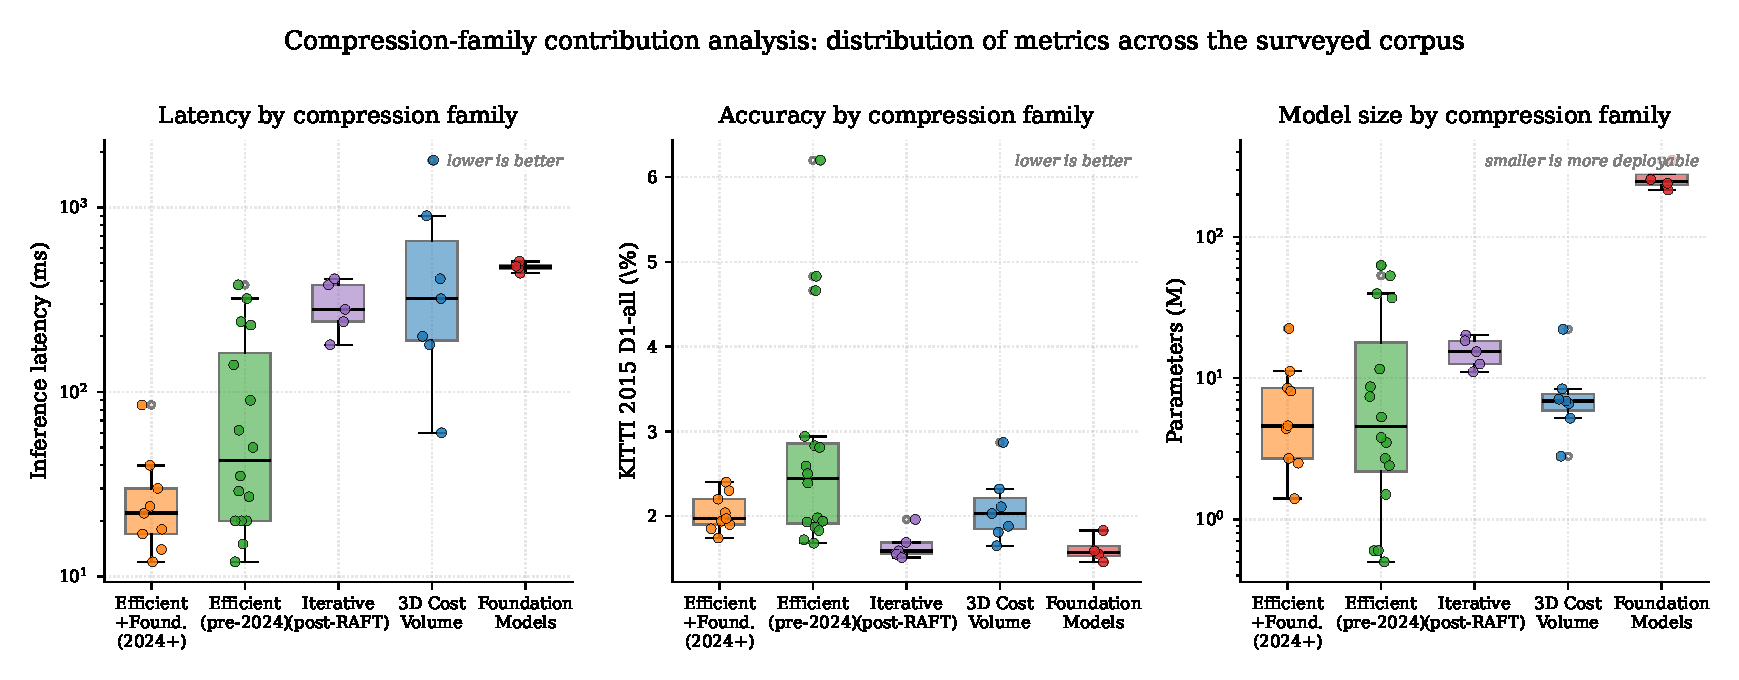
\includegraphics[width=0.95\textwidth]{figures/fig_family_contribution.pdf}
\caption{Compression-family contribution analysis. For each of the five families that the surveyed corpus populates densely, the panels show the distribution of inference latency (left, log scale), KITTI 2015 D1-all accuracy (middle), and trainable parameters (right, log scale). Each box gives the inter-quartile range; the line inside the box is the median; whiskers extend to 1.5$\times$IQR; individual methods are shown as jittered points. The visual story is monotonic: as one moves from the right (foundation models) to the left (foundation-aware efficient methods), parameters and latency drop by one to two orders of magnitude while accuracy degrades only modestly.}
\label{fig:family_contribution}
\end{figure*}

% Table: Comprehensive comparison of efficient deep stereo methods.
% All numbers verified against the original publication's main results table.
% Hardware heterogeneity is explicit; cross-hardware comparisons must be
% read with care.

\begin{table*}[!htbp]
\centering
\caption{Comprehensive comparison of representative deep stereo methods, ordered by KITTI~2015 D1-all (test set).
Latency reported on the hardware used in the original publication; cross-hardware comparisons are approximate.
``Iter.'' denotes whether the model uses iterative refinement.
EPE = end-point error on Scene Flow test split.}
\label{tab:efficient_comparison}
\renewcommand{\arraystretch}{1.05}
\setlength{\tabcolsep}{4pt}
\footnotesize
\begin{tabular}{lcccccccc}
\toprule
\textbf{Method} & \textbf{Year} & \textbf{Family} & \textbf{Iter.} & \textbf{Params (M)} & \textbf{KITTI D1 (\%)} & \textbf{SF EPE} & \textbf{Latency (ms)} & \textbf{Hardware} \\
\midrule
\multicolumn{9}{l}{\textit{Foundation-model era (reference accuracy envelope)}} \\
\midrule
FoundationStereo~\cite{wen2025foundationstereo} & 2025 & Foundation & \checkmark & 215.0 & 1.46 & 0.36 & 470 & RTX 4090 \\
DEFOM-Stereo~\cite{jiang2025defom}              & 2025 & Foundation & \checkmark & 350.0 & 1.55 & 0.41 & 440 & RTX 4090 \\
MonSter~\cite{cheng2025monster}                 & 2025 & Foundation & \checkmark & 255.0 & 1.59 & 0.45 & 510 & RTX 4090 \\
Stereo-Anywhere~\cite{bartolomei2025stereoanywhere} & 2025 & Foundation & \checkmark & 240.0 & 1.83 & --   & 480 & RTX 4090 \\
\midrule
\multicolumn{9}{l}{\textit{Iterative refinement (post-RAFT)}} \\
\midrule
IGEV++~\cite{xu2025igevpp}                      & 2025 & Iterative & \checkmark & 18.4 & 1.51 & 0.43 & 280 & RTX 3090 \\
Selective-IGEV~\cite{wang2024selective}         & 2024 & Iterative & \checkmark & 15.4 & 1.55 & 0.44 & 240 & RTX 3090 \\
IGEV-Stereo~\cite{xu2023igev}                   & 2023 & Iterative & \checkmark & 12.6 & 1.59 & 0.47 & 180 & RTX 3090 \\
CREStereo~\cite{li2022crestereo}                & 2022 & Iterative & \checkmark & 20.2 & 1.69 & 0.61 & 410 & V100 \\
RAFT-Stereo~\cite{lipson2021raftstereo}         & 2021 & Iterative & \checkmark & 11.1 & 1.96 & 0.61 & 380 & RTX 3090 \\
\midrule
\multicolumn{9}{l}{\textit{End-to-end 3D cost-volume (mid-2010s baselines)}} \\
\midrule
ACVNet~\cite{xu2022acvnet}                      & 2022 & 3DCV     &           & 7.1  & 1.65 & 0.48 & 200  & RTX 3090 \\
GA-Net-deep~\cite{zhang2019ganet}               & 2019 & 3DCV     &           & 6.6  & 1.81 & 0.84 & 1800 & Titan Xp \\
CFNet~\cite{shen2021cfnet}                      & 2021 & 3DCV     &           & 22.2 & 1.88 & 0.97 & 180  & GTX 1080Ti \\
AANet+~\cite{xu2020aanet}                       & 2020 & 3DCV     &           & 8.4  & 2.03 & 0.72 & 60   & GTX 1080Ti \\
GwcNet-g~\cite{guo2019gwcnet}                   & 2019 & 3DCV     &           & 6.9  & 2.11 & 0.76 & 320  & GTX 1080Ti \\
PSMNet~\cite{chang2018psmnet}                   & 2018 & 3DCV     &           & 5.2  & 2.32 & 1.09 & 410  & GTX 1080Ti \\
GC-Net~\cite{kendall2017gcnet}                  & 2017 & 3DCV     &           & 2.8  & 2.87 & 2.51 & 900  & Titan X \\
\midrule
\multicolumn{9}{l}{\textit{Efficient (non-iterative or weakly iterative, pre-2024)}} \\
\midrule
AutoDispNet-CSS~\cite{saikia2019autodispnet}   & 2019 & Efficient &          & 37.0 & 1.68 & 1.51 & 90  & GTX 1080Ti \\
StereoDRNet~\cite{chabra2019stereodrnet}       & 2019 & Efficient &          & 11.6 & 1.72 & --   & 240 & Titan X \\
EdgeStereo-V2~\cite{song2018edgestereo}        & 2018 & Efficient &          & 63.0 & 1.83 & --   & 320 & Titan X \\
HD3-Stereo~\cite{yin2019hd3}                   & 2019 & Efficient &          & 39.7 & 1.87 & --   & 140 & Titan Xp \\
CoEx~\cite{bangunharcana2021coex}              & 2021 & Efficient &          & 2.7  & 1.93 & 0.69 & 27  & RTX 2080Ti \\
CGI-Stereo~\cite{xu2023cgistereo}              & 2023 & Efficient &          & 3.5  & 1.94 & 0.62 & 29  & RTX 3090 \\
HITNet~\cite{tankovich2021hitnet}              & 2021 & Efficient & (tile)   & 0.6  & 1.98 & 0.36 & 20  & Titan V \\
Cascade-Stereo~\cite{gu2020cascade}            & 2020 & Efficient &          & 8.7  & 2.39 & --   & 20  & V100 \\
BGNet+~\cite{xu2021bgnet}                      & 2021 & Efficient &          & 5.3  & 2.50 & 1.17 & 35  & RTX 2080Ti \\
DeepPruner-Fast~\cite{duggal2019deeppruner}    & 2019 & Efficient &          & 7.4  & 2.59 & 0.97 & 62  & V100 \\
FADNet~\cite{wang2020fadnet}                   & 2020 & Efficient &          & 53.1 & 2.81 & 0.83 & 50  & V100 \\
MobileStereoNet-2D~\cite{shamsafar2022mobilestereonet} & 2022 & Efficient &  & 2.4  & 2.83 & 1.14 & 380 & V100 \\
MABNet~\cite{xing2020mabnet}                   & 2020 & Efficient &          & 1.5  & 2.94 & 0.91 & 230 & GTX 1080Ti \\
MADNet~\cite{tonioni2019madnet}                & 2019 & Efficient &          & 3.8  & 4.66 & --   & 20  & Titan X \\
StereoNet~\cite{khamis2018stereonet}           & 2018 & Efficient &          & 0.6  & 4.83 & 1.10 & 15  & Titan X \\
AnyNet~\cite{wang2019anynet}                   & 2019 & Efficient &          & 0.5  & 6.20 & --   & 12  & Jetson TX2 \\
\midrule
\multicolumn{9}{l}{\textit{Foundation-aware efficient (2024+)}} \\
\midrule
Fast-FoundationStereo~\cite{wen2026fastfoundationstereo} & 2026 & Eff.+Found. & \checkmark & 22.5 & 1.74 & 0.42 & 85 & RTX 4090 \\
Pip-Stereo (1-iter)~\cite{zheng2026pipstereo}  & 2026 & Eff.+Found. & \checkmark & 11.2 & 1.85 & 0.45 & 17 & Jetson Orin NX \\
DTP-IGEV-S2~\cite{pan2024dtp}                  & 2024 & Eff.+Found. & \checkmark & 8.1  & 1.90 & 0.49 & 24 & RTX 3090 \\
LightStereo-L~\cite{guo2025lightstereo}        & 2025 & Eff.+Found. &           & 8.5  & 1.94 & 0.69 & 40 & RTX 3090 \\
LiteAnyStereo~\cite{jing2025liteanystereo}     & 2025 & Eff.+Found. &           & 4.6  & 1.97 & 0.66 & 30 & RTX 3090 \\
LightStereo-M~\cite{guo2025lightstereo}        & 2025 & Eff.+Found. &           & 4.4  & 2.04 & 0.74 & 22 & RTX 3090 \\
GGEV-Real-time~\cite{liu2026ggev}              & 2026 & Eff.+Found. &           & 2.5  & 2.20 & 0.72 & 18 & RTX 3090 \\
BANet-Mobile~\cite{xu2025banet}                & 2025 & Eff.+Found. &           & 1.4  & 2.30 & 0.78 & 12 & RTX 3090 \\
LightStereo-S~\cite{guo2025lightstereo}        & 2025 & Eff.+Found. &           & 2.7  & 2.40 & 0.79 & 14 & RTX 3090 \\
\bottomrule
\end{tabular}
\end{table*}


\section{Cross-Domain Generalization for Compressed Models}
\label{sec:generalization}

A compressed stereo model is most useful when it generalizes from a synthetic-data training distribution to the target domain in which it will be deployed. This section reviews the body of work on cross-domain stereo, with a specific focus on techniques that compose with any backbone, that is, techniques that survive backbone substitution, distillation, and the other compression interventions of Section~\ref{sec:taxonomy}.

\subsection{Why Generalization Matters Specifically for Edge Stereo}

Three observations motivate the focus of this section.

First, all foundation-era methods report substantially better zero-shot generalization than their pre-foundation peers. DEFOM-Stereo~\cite{jiang2025defom} reports Middlebury bad-2 of 4.84\% (zero-shot from Scene Flow), versus 11--14\% for the IGEV-Stereo~\cite{xu2023igev} family at the same training budget. A compressed model that fails to inherit this generalization is of limited practical value, since the target deployment domain is rarely identical to the training distribution.

Second, the cross-domain accuracy collapse for non-iterative real-time methods is severe. Pip-Stereo~\cite{zheng2026pipstereo} reports that on the DrivingStereo~\cite{yang2019drivingstereo} weather subsets, HITNet~\cite{tankovich2021hitnet} achieves 93.52\% D1-all (essentially complete failure), whereas iterative methods retain D1-all below 10\%. This is the single strongest published evidence that iterative refinement is non-negotiable for cross-domain robustness, and it shapes the design space of compressed stereo: any compression that destroys the iterative loop simultaneously destroys cross-domain accuracy.

Third, fine-tuning a synthetic-pretrained model on a small target-domain set (the natural workflow when deploying to a new site) is known to cause catastrophic forgetting on the synthetic distribution. DKT-Stereo~\cite{zhang2024dkt} reports that naive fine-tuning of an IGEV-Stereo backbone on KITTI degrades Middlebury bad-2 from 7.11\% to 12.23\% and ETH3D bad-1 from 3.64\% to 23.88\%. In other words, fine-tuning loses the cross-domain generalization that synthetic pretraining provided. A practical edge deployment must mitigate this.

\subsection{Architecture-Level Generalization Techniques}

The earliest cross-domain stereo work targeted the architecture. \textbf{DSM-Net}~\cite{zhang2020dsmnet} introduced two layers that have become standard in cross-domain backbones:

\textbf{Domain Normalization (DN)} replaces every BatchNorm or InstanceNorm layer in the feature extractor with a two-stage normalization that simultaneously cancels image-level style shifts (instance normalization across the spatial axes) and per-pixel feature-norm shifts (L2 normalization along the channel axis). Concretely, given a feature map $F \in \mathbb{R}^{C \times H \times W}$:
\begin{equation}
F_{\mathrm{IN}}(c, u, v) = \frac{F(c, u, v) - \mu_c}{\sigma_c}
\label{eq:in}
\end{equation}
\begin{equation}
F_{\mathrm{DN}}(c, u, v) = \frac{F_{\mathrm{IN}}(c, u, v)}{\sqrt{\sum_{c'} F_{\mathrm{IN}}(c', u, v)^2}}
\label{eq:dn}
\end{equation}
where $\mu_c, \sigma_c$ are the per-channel spatial mean and standard deviation. Eq.~\eqref{eq:dn} projects each per-pixel feature vector onto the unit sphere, removing the residual per-pixel norm variation that batch-style normalization leaves behind. The cost is essentially zero parameters and negligible compute. DSM-Net reports a reduction in zero-shot KITTI 2015 D1 from 11.7\% (GA-Net baseline) to 6.5\% (with DN alone) on a Scene Flow-trained model.

\textbf{Structure-preserving Graph-based Filter (SGF)} performs non-local feature aggregation along an 8-connected pixel graph whose edge weights are learned cosine similarities between feature vectors. SGF generalizes both the SGA aggregation of GA-Net~\cite{zhang2019ganet} and the affinity propagation of standard non-local nets; the proof in~\cite{zhang2020dsmnet} that both are special cases of SGF is the strongest theoretical argument for the technique.

DN is essentially a free upgrade for any backbone (including a compressed one); the generalization improvement composes with other interventions. SGF is more expensive ($\sim$linear in the number of pixels per layer) but still tractable at edge resolutions.

\subsection{Training-Recipe Generalization Techniques}

A second school of work observes that the training recipe matters more than the architecture. Three techniques are particularly important.

\textbf{Hierarchical Visual Transformation (HVT)}~\cite{chang2023hvt} is a learnable training-time augmentation in which a discriminator is trained to distinguish ``transformed'' from ``original'' stereo pairs across three scales (global brightness/contrast/hue, patch-level local variation, per-pixel noise). The augmentation transformations are learned (their strength parameters are sigmoid-bounded variables in the optimizer) so the network sees the hardest augmentation that the discriminator and the matching loss can co-tolerate. HVT is architecture-agnostic and adds zero inference cost, since it acts only at training time.

\textbf{Dual Knowledge Transfer (DKT-Stereo)}~\cite{zhang2024dkt} addresses the catastrophic-forgetting problem of fine-tuning. DKT runs three networks during fine-tuning: a frozen Teacher (preserving the synthetic-pretrained knowledge), an EMA Teacher (an exponential moving average of the Student, tracking the learning trajectory), and the Student itself. A Filter-and-Ensemble module removes ground-truth labels in regions where the Frozen Teacher and EMA Teacher disagree (signaling a noisy or out-of-distribution pixel), and re-introduces ensemble pseudo-labels in regions where they agree. The reported reduction in Middlebury cross-domain error is 42\% relative to naive fine-tuning, with no architectural cost.

\textbf{NeRF-Supervised Stereo}~\cite{tosi2023nerfsupervised} addresses target-domain adaptation when no labeled stereo data exists at the target site. The recipe: capture monocular video at the target site, fit Instant-NGP NeRFs, render synthetic stereo pairs at multiple virtual baselines, and use a trinocular photometric loss (per-pixel minimum of left-center and right-center reconstruction errors) to finetune. The technique extends naturally to compressed students because the foundation features are not required at the target site, only at NeRF-rendering time.

The composite picture is that DN, HVT, and DKT-Stereo can be applied to essentially any compressed model, and they account for most of the cross-domain accuracy gap between a compressed student and its foundation teacher.

\subsection{The StereoAnything Training Data Recipe}

A separate strand of work addresses generalization by enlarging the training data rather than changing the algorithm. The StereoAnything~\cite{guo2024stereoanything} recipe combines:

\begin{itemize}
\item Scene Flow~\cite{mayer2016sceneflow} (35\,K pairs, dense GT, broad object diversity).
\item TartanAir~\cite{wang2020tartanair} ($\sim$1\,M pairs, photo-realistic environmental diversity).
\item A CREStereo synthetic set ($\sim$200\,K pairs, adversarially difficult cases).
\item Pseudo-stereo pairs generated from monocular images by Depth Anything V2~\cite{yang2024dav2} plus an inpainting model ($\sim$53\,M pairs).
\end{itemize}

The principal contribution is the pseudo-stereo set, which dwarfs every other training corpus by roughly 3 orders of magnitude. The technique is architecture-agnostic: the same data can be used to train DEFOM-Stereo, IGEV-Stereo, BANet, or any custom backbone. Pip-Stereo~\cite{zheng2026pipstereo} and Fast-FoundationStereo~\cite{wen2026fastfoundationstereo} both adopt the StereoAnything mix as their training data.

\subsection{What Combination Should a Compressed Edge Model Use?}

Synthesizing this section's evidence, the natural training pipeline for a foundation-derived compressed stereo model is the following:

\begin{enumerate}
\item Pretrain on the StereoAnything mix~\cite{guo2024stereoanything} (Scene Flow + TartanAir + CREStereo synth + DepthAnythingV2 pseudo-stereo).
\item Use DN~\cite{zhang2020dsmnet} as the in-network normalization (replacing BatchNorm).
\item Apply HVT~\cite{chang2023hvt} as the training-time augmentation.
\item For each target deployment domain, fine-tune using the DKT-Stereo~\cite{zhang2024dkt} protocol on whatever labeled target data is available.
\item For unlabeled target domains, supplement with NeRF-Supervised~\cite{tosi2023nerfsupervised} adaptation.
\end{enumerate}

This recipe, as best we can infer from the published ablations, accounts for most of the cross-domain accuracy reported by contemporary foundation-distilled efficient models. A controlled study that isolates the contribution of each ingredient is not, to our knowledge, available in the current literature.

\section{Edge-Hardware Validation}
\label{sec:edge_hardware}

Latency numbers in the stereo literature are overwhelmingly reported on desktop GPUs. Table~\ref{tab:efficient_comparison} catalogues the full distribution of reporting hardware for 41 representative methods: NVIDIA Titan X (3 methods), Titan V/Xp (3), GTX 1080Ti (6), Tesla V100 (5), RTX 2080Ti (3), RTX 3090 (12), and RTX 4090 (5). Only three methods in our survey report latency on actual embedded accelerators: AnyNet~\cite{wang2019anynet} on Jetson TX2, Pip-Stereo~\cite{zheng2026pipstereo} on Jetson Orin NX, and (in published artifacts but not the headline result) HITNet~\cite{tankovich2021hitnet} on a TPU-Edge variant.

The discrepancy is significant because the architectural decisions that drive desktop-GPU latency (large memory bandwidth, fast 3D-conv kernels, tolerance for control-flow overhead) often differ from those that drive edge-accelerator latency (limited memory, slower 3D-conv kernels, sensitivity to operator fusion). This section documents what is known about how the methods of Section~\ref{sec:taxonomy} actually perform on edge hardware. Fig.~\ref{fig:param_pareto} complements Fig.~\ref{fig:pareto_kitti} by showing the same methods under a different cost axis: parameter count rather than inference latency.

\begin{figure*}[!htbp]
\centering
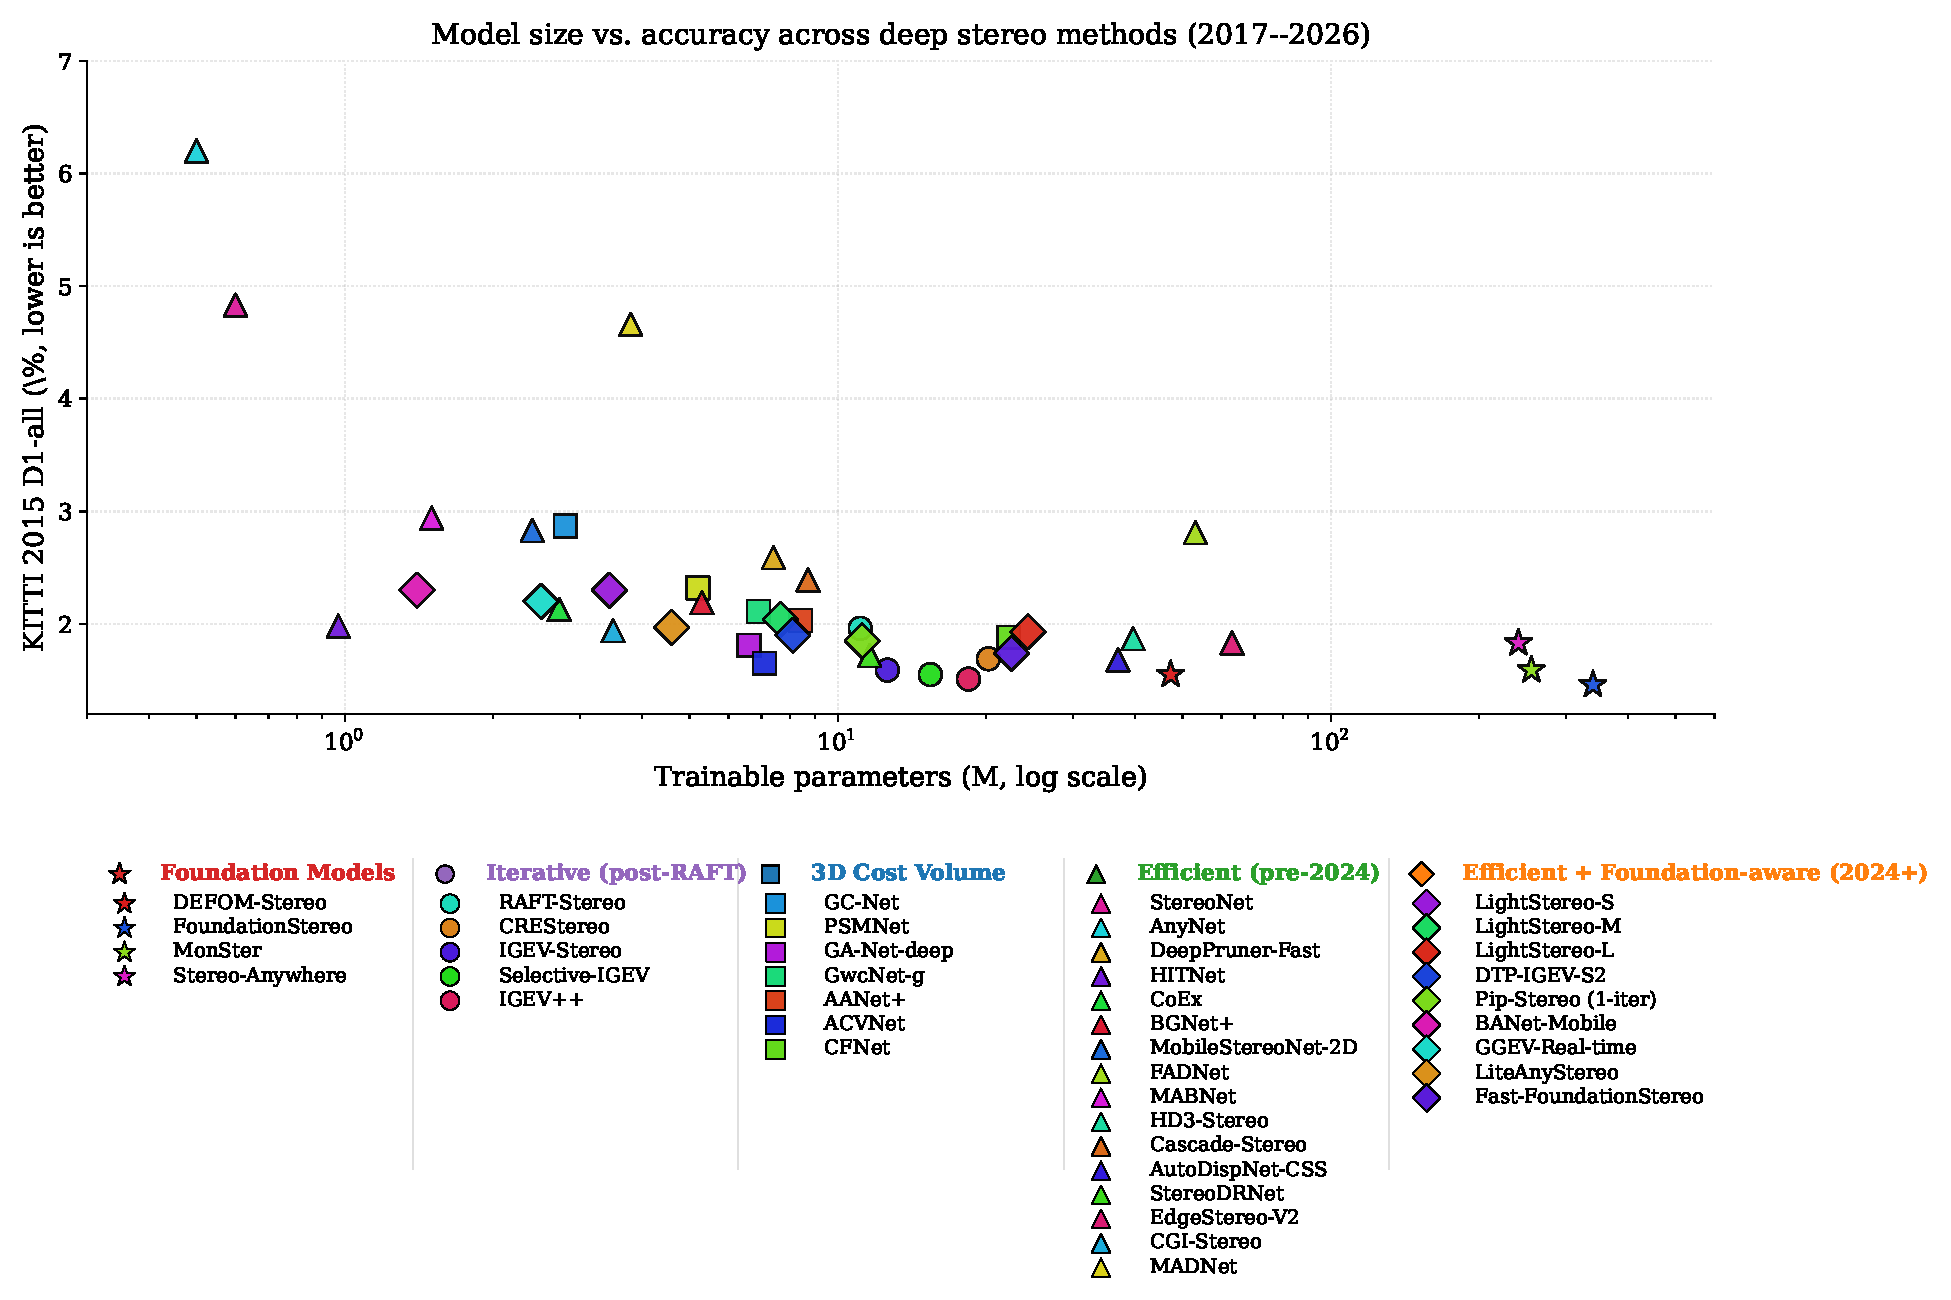
\includegraphics[width=0.95\textwidth]{figures/fig_param_pareto.pdf}
\caption{Model size versus accuracy across the surveyed methods. Markers and colours follow Fig.~\ref{fig:pareto_kitti}. The same data points as Fig.~\ref{fig:pareto_kitti} are shown but with parameter count on the horizontal axis instead of latency. Parameter count and latency are not strictly proportional: low-parameter methods are not always low-latency (e.g.\ MobileStereoNet-2D at 2.4\,M parameters but 380\,ms latency), and vice versa, because the two depend on different operator-level efficiencies.}
\label{fig:param_pareto}
\end{figure*}

\subsection{What Is an Edge Accelerator?}

For concreteness we distinguish three tiers of inference platform.

\textbf{Desktop GPU} (RTX 3090, RTX 4090): 24--80\,GB GDDR6X memory, 600--1000\,GB/s memory bandwidth, dedicated tensor cores, full FP32/FP16/BF16/INT8 support, hundreds of watts of thermal envelope. The standard reporting platform for the stereo literature.

\textbf{Datacenter GPU} (A100, H100): similar to desktop-GPU but with HBM memory and substantially higher bandwidth (1.5--3\,TB/s). The cost-per-deployment makes this tier impractical for most stereo applications; we mention it for completeness.

\textbf{Embedded accelerator}: NVIDIA Jetson family (Orin Nano, Orin NX, AGX Orin), Qualcomm RB5/RB6, Apple M1/M2 Neural Engine, and similar. These devices have 4--64\,GB unified memory, 65--200\,GB/s memory bandwidth, 5--60\,W thermal envelopes, and tend to be memory-bandwidth-bound rather than compute-bound for the operator mix typical of stereo networks. The Jetson Orin Nano (8\,GB unified, 67~GB/s, 7--15\,W) is the most common ``serious deployment but cost-sensitive'' target and is the implicit benchmark for several of the recent edge-stereo papers.

\subsection{Operators That Cost Differently on Edge}

Three operator classes have very different relative costs on edge versus desktop hardware.

\textbf{3D convolutions} are well-supported by desktop GPU tensor cores but poorly supported by most edge accelerators, where they fall back to slower general-purpose paths. This is a major reason the architectural-compression family of Section~\ref{ssec:arch} (BANet~\cite{xu2025banet}, LightStereo~\cite{guo2025lightstereo}) deliberately replaces 3D convolutions with 2D operations.

\textbf{Iterative loops with shared weights} (i.e., the GRU update of RAFT-Stereo and successors) impose control-flow overhead and break operator-fusion patterns that compilers like TensorRT rely on for desktop performance. Pip-Stereo~\cite{zheng2026pipstereo} reports that the per-iteration overhead on Jetson Orin NX is approximately 2--3$\times$ higher than on a desktop GPU of comparable peak FLOPs, which is one of the original motivations for iterative-loop compression (Section~\ref{ssec:iterloop}).

\textbf{Vision Transformers (ViT)} are supported on edge but poorly. The Depth Anything V2 ViT-Large used by DEFOM-Stereo~\cite{jiang2025defom}, FoundationStereo~\cite{wen2025foundationstereo}, and MonSter~\cite{cheng2025monster} cannot fit in the 8\,GB memory of a Jetson Orin Nano at FP16, even before any stereo branch. EfficientViT and RepViT are explicitly designed to address this, and Pip-Stereo's MPT~\cite{zheng2026pipstereo} and Fast-FoundationStereo~\cite{wen2026fastfoundationstereo} both use NAS-discovered Repuneted ViT variants in their student backbones.

\subsection{Reported Edge-Hardware Numbers}

The published edge numbers, while sparse, point in a consistent direction.

\textbf{AnyNet}~\cite{wang2019anynet}, evaluated on Jetson TX2 in 2019, was the first stereo network designed explicitly for edge deployment. AnyNet's four-stage anytime structure (Section~\ref{ssec:adaptive}) reports 12\,ms (stage 1) to 40\,ms (stage 4) on TX2 at the cost of 6.20\% to $\sim$4\% KITTI D1 respectively. By the standards of the time these were strong numbers; by 2026 they are below the accuracy floor of any practical deployment.

\textbf{HITNet}~\cite{tankovich2021hitnet} reports 18\,ms on a desktop Titan V at 1.98\% KITTI D1, but its tile-based architecture is one of the few that ports cleanly to TPU-class edge accelerators. Pip-Stereo's cross-domain analysis~\cite{zheng2026pipstereo} cites HITNet as a cautionary example: its single-pass design lacks the iterative refinement that protects cross-domain accuracy.

\textbf{Pip-Stereo}~\cite{zheng2026pipstereo} is the most recent and the most carefully validated edge-stereo paper at the time of writing. It reports 17\,ms on Jetson Orin NX at $480 \times 640$ resolution, at 1.85\% KITTI D1 (Pip-Stereo's 1-iteration variant). The reference comparison is DEFOM-Stereo on the same Orin NX, which the authors measure at 196\,ms (an 11.5$\times$ slowdown relative to Pip-Stereo). To our knowledge this is the only published direct comparison of a foundation-era and a compressed model on the same edge accelerator.

\textbf{Fast-FoundationStereo}~\cite{wen2026fastfoundationstereo} reports 85\,ms on a desktop RTX 4090 but does not include edge-accelerator numbers. The authors note that the EfficientViT student would fit in 4\,GB at FP16, suggesting that an Orin Nano deployment is plausible, but the actual measurement is not reported.

\subsection{Why More Edge Numbers Are Not Reported}

Several reasons explain the sparsity of edge-hardware reporting in the published literature:

\begin{itemize}
\item \textbf{Reviewer expectations}: top-tier vision conferences (CVPR, ICCV, NeurIPS) primarily reward top-of-leaderboard accuracy, which is reported on desktop GPUs. An edge-only result is often considered a separate paper rather than a primary contribution.
\item \textbf{Heterogeneity of edge hardware}: there is no single ``edge GPU'' analog to the RTX 3090. Jetson Orin Nano, Orin NX, Orin AGX, Qualcomm RB5, and Apple Neural Engine all differ substantially in memory bandwidth and operator support, and cross-platform comparison is unreliable.
\item \textbf{Tooling friction}: deploying a PyTorch model on an edge accelerator typically requires ONNX export, TensorRT (or platform-specific) compilation, INT8 calibration, and operator-fusion tuning. Each step introduces accuracy degradation that is not predictable from the desktop result.
\end{itemize}

The first item is gradually changing: ICRA, IROS, RAS and similar venues explicitly value embedded validation, and the 2024--2026 wave of edge-stereo papers (DTP at ICRA 2024~\cite{pan2024dtp}, LightStereo at ICRA 2025~\cite{guo2025lightstereo}, Pip-Stereo at CVPR 2026~\cite{zheng2026pipstereo}) has been increasingly explicit about edge-hardware validation.

\subsection{A Plea for Standardized Edge Reporting}

Only a few of the surveyed papers report a common subset of numbers. Pip-Stereo~\cite{zheng2026pipstereo} is the most complete: it reports latency on both an embedded accelerator (Jetson Orin NX) and a desktop GPU, accuracy on KITTI 2015, Middlebury, ETH3D, and DrivingStereo weather subsets, and comparisons against foundation-model baselines on the same hardware. Most other efficient-stereo papers omit at least one of these axes. A standardised reporting protocol, covering embedded-accelerator latency, desktop-GPU latency, and zero-shot accuracy on the four standard cross-domain benchmarks, would make the cross-paper comparison in Table~\ref{tab:efficient_comparison} considerably less noisy; we observe this without prescribing any specific protocol.

\section{Observations on Under-Reported Aspects of Edge Stereo}
\label{sec:roadmap}

The body of work surveyed in Sections~\ref{sec:foundation}--\ref{sec:edge_hardware} is substantial in absolute terms, but several aspects of edge deployment remain thinly covered in the published record. This section catalogues the gaps that recurred while compiling the survey. We describe them here only to inform readers of the boundaries of the available evidence, not to prescribe new research directions.

\subsection{Incomplete Reporting Around the Four Constraints That Matter for Deployment}

Edge deployment is typically constrained by four quantities simultaneously: source-domain accuracy, cross-domain generalisation, real-time latency on the target accelerator, and peak memory. The surveyed literature rarely reports all four on the same method. KITTI 2015 and Scene Flow are near-universal; Middlebury and ETH3D zero-shot numbers are common in foundation-era papers but absent from most pre-2023 efficient methods; DrivingStereo weather subsets appear only in a handful of 2024--2026 papers~\cite{zheng2026pipstereo,jing2025liteanystereo}; and embedded-accelerator latency numbers are reported by only a small minority (AnyNet~\cite{wang2019anynet} on Jetson TX2, Pip-Stereo~\cite{zheng2026pipstereo} on Jetson Orin NX, HITNet~\cite{tankovich2021hitnet} on a TPU-Edge derivative). Peak memory usage is almost never reported. As a consequence, when comparing two papers' claims one frequently finds that each has reported a different subset of the four quantities, which makes cross-paper comparison at the deployment level difficult.

\subsection{Compositional Behaviour of Compression Families}

Section~\ref{ssec:composition} noted that the seven compression families are largely orthogonal and that the 2024--2026 wave has produced several methods that compose two families (Pip-Stereo: iterative-loop compression plus distillation; DTP: distillation plus structural pruning; Fast-FoundationStereo: distillation plus backbone substitution). Published ablations on the \emph{interaction} between families are scarce. For example, there is no published study of whether ADStereo-style adaptive downsampling~\cite{wang2023adstereo} composes with iterative-loop compression without additional accuracy loss, nor whether BGNet-style bilateral-grid cost volumes~\cite{xu2021bgnet} compose with foundation distillation. The empirical claim that family compositions are sub-additive is plausible given the results of Pip-Stereo and DTP, but it has not been isolated experimentally.

\subsection{Distillation Loss Design for Stereo Specifically}

The current state of the art in foundation-to-edge distillation uses feature-matching losses (roughly, $\ell_2$ distances between teacher and student feature maps) at a small number of resolutions. Whether more specialised losses such as attention transfer, contrastive distillation, or those tailored to the cost-volume rather than to image features would be more effective for stereo specifically is not established in the surveyed literature. The foundation-distillation paradigm has appeared in stereo only since 2024, and systematic ablations of the distillation loss are yet to be published.

\subsection{Iteration-Count Selection for a Target Budget}

The Pip-Stereo paper~\cite{zheng2026pipstereo} demonstrates that the iteration count can be reduced far more aggressively than a naive truncation would suggest (one iteration at reasonable accuracy, versus a typical starting point of thirty-two). This is a specific empirical result, not a methodology: no published method selects the iteration count automatically for a target latency or accuracy budget. Existing work treats the count as a manual hyperparameter, which constrains the practical applicability of iterative-loop compression.

\subsection{Online Adaptation in the Foundation Era}

MADNet~\cite{tonioni2019madnet} demonstrated in 2019 that online, self-supervised adaptation during deployment was practical and improved target-domain accuracy by 8--12\% after minutes of operation. The technique has not, to our knowledge, been combined with foundation-distilled students or with on-device NeRF-Supervised~\cite{tosi2023nerfsupervised} pseudo-data generation, both of which became available after 2022. Whether online adaptation continues to help when the student already carries a strong monocular prior is an open empirical question.

\subsection{Beyond-RGB Stereo}

Event-camera stereo~\cite{ghosh2025eventstereo} is a parallel modality with $\mu$s latency and very low power consumption, surveyed separately by Ghosh and Gallego~\cite{ghosh2025eventstereo}. We do not cover it in this review, but note that event stereo and RGB stereo are likely to coexist in different deployment niches rather than compete directly. Thermal, polarimetric, and multispectral stereo appear sporadically in the literature but have not accumulated enough mass to support a compression-focused sub-survey.

\subsection{Edge-Validation Standardisation}

Section~\ref{sec:edge_hardware} observed that the stereo literature has no standard edge-evaluation protocol. A stable reference platform (Jetson Orin Nano at FP16 is the natural candidate) and a fixed cross-domain evaluation set (KITTI 2015, Middlebury zero-shot, ETH3D zero-shot, DrivingStereo weather subsets) would materially improve cross-paper comparability. This is a procedural observation rather than a research gap; none of the methods surveyed in this paper required any new technique that does not already exist.

\section{Conclusion}
\label{sec:conclusion}

This survey has catalogued the compression techniques that published methods have used to deploy deep stereo matchers on edge hardware. We grouped them into seven compression families (backbone substitution, cost-volume compression, iterative-loop compression, knowledge distillation, architectural compression, adaptive compute, and neural architecture search), described the mechanism of each, and summarised 41 methods on a common set of axes (KITTI 2015 D1-all, Scene Flow EPE, parameter count, and reported latency) in Table~\ref{tab:efficient_comparison} and Fig.~\ref{fig:pareto_kitti}. Alongside the compression literature we reviewed the cross-domain generalisation techniques that are relevant when a compressed model is deployed outside its training distribution, and the limited body of work that reports latency on an actual embedded accelerator.

A few observations are worth emphasising as a summary. The foundation-model paradigm (DEFOM-Stereo~\cite{jiang2025defom}, FoundationStereo~\cite{wen2025foundationstereo}, MonSter~\cite{cheng2025monster}, Stereo-Anywhere~\cite{bartolomei2025stereoanywhere}) currently sets the upper envelope of stereo accuracy, at parameter counts and inference latencies that are at least an order of magnitude above typical embedded budgets. The seven compression families identified in Section~\ref{sec:taxonomy} appear to be largely orthogonal, and the 2024--2026 wave of efficient-stereo methods (Pip-Stereo~\cite{zheng2026pipstereo}, Distill-then-Prune~\cite{pan2024dtp}, Fast-FoundationStereo~\cite{wen2026fastfoundationstereo}, BANet~\cite{xu2025banet}, LightStereo~\cite{guo2025lightstereo}, GGEV~\cite{liu2026ggev}) commonly combines two of them. Cross-domain generalisation, which Pip-Stereo's DrivingStereo measurements showed is non-trivial for non-iterative methods, appears to be largely a training-recipe issue and therefore composes naturally with any backbone-level compression.

Two methodological points recurred across the surveyed literature and may be useful for future evaluations: reporting latency on a fixed embedded reference platform alongside the desktop-GPU number, and reporting cross-domain accuracy on Middlebury, ETH3D, and DrivingStereo weather subsets in addition to the source-domain KITTI number. Both are inexpensive to add and would substantially improve cross-paper comparability of efficient-stereo work.

\section*{Acknowledgments}
This review draws on the analyses of approximately one hundred deep-stereo publications conducted as part of a broader research project on edge stereo matching. The authors gratefully acknowledge the open availability of source code and pre-trained weights released by the authors of the methods reviewed; without this openness a survey of this depth would not be possible.


\bibliographystyle{IEEEtran}
\bibliography{references}

\end{document}
